\chapter{Umsetzung}
\label{chapter:implementation}
    
    \todo{Frontend und Backend ist nur ein einfacher Vergleich zwischen Mockup und wie es tatsächlich aussieht.
          Da sollten evtl. noch Details zur Implementierung rein, evtl. Probleme, usw.}

    In diesem Kapitel wird die Umsetzung des System erläutert.
    Zunächst wird die zur Implementierung verwendete Software näher erläutert.
    Anschließend werden Front- und Backend kurz vorgestellt und mit dem Entwurf aus Kapitel \ref{chapter:design} verglichen.
    
    \section{Verwendete Software}
        Die in Kapitel \ref{chapter:requirements} vorgestellte Software wurde verwendet.
        \todo{Text von irgendjemanden der Ahnung hat\\}
        
    \section{Frontend}
        Die Entwürfe für das Frontend wurden ohne große Änderungen umgesetzt.
        
        \begin{figure}
            \centering
            \begin{subfigure}{0.4\textwidth}
                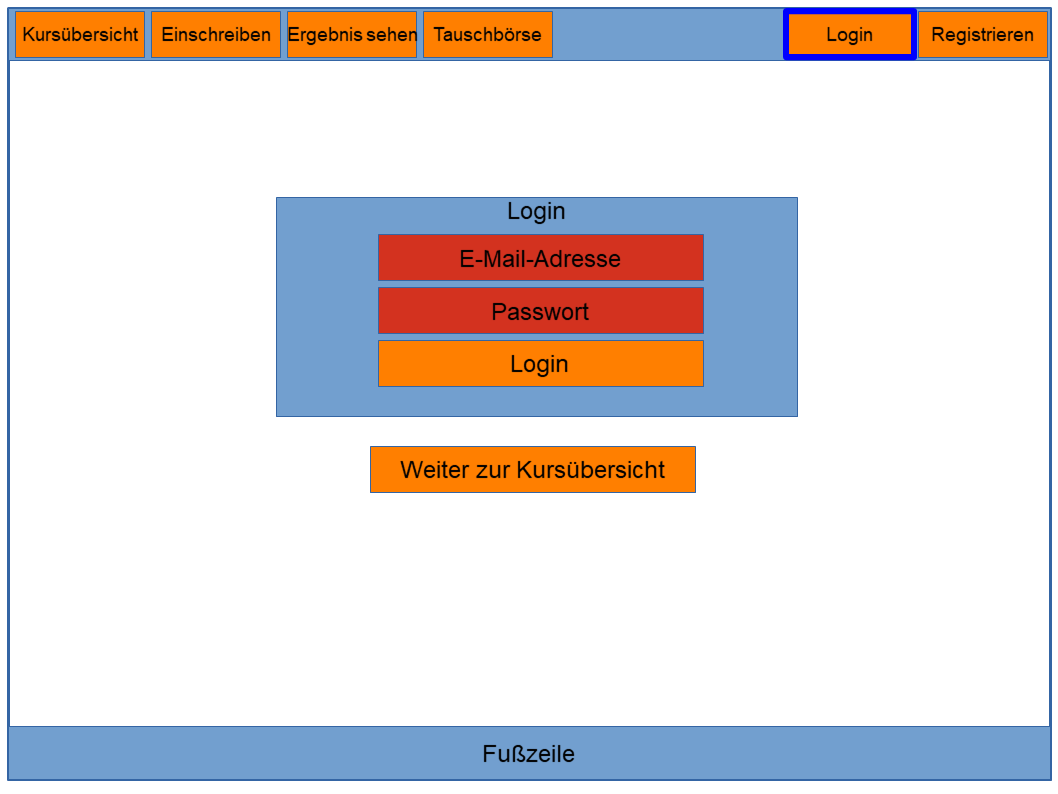
\includegraphics[width=1.0\textwidth]{./implementation/images/MockUpsFrontend/frontendLogin.png}
            \end{subfigure}
            \begin{subfigure}{0.59\textwidth}
                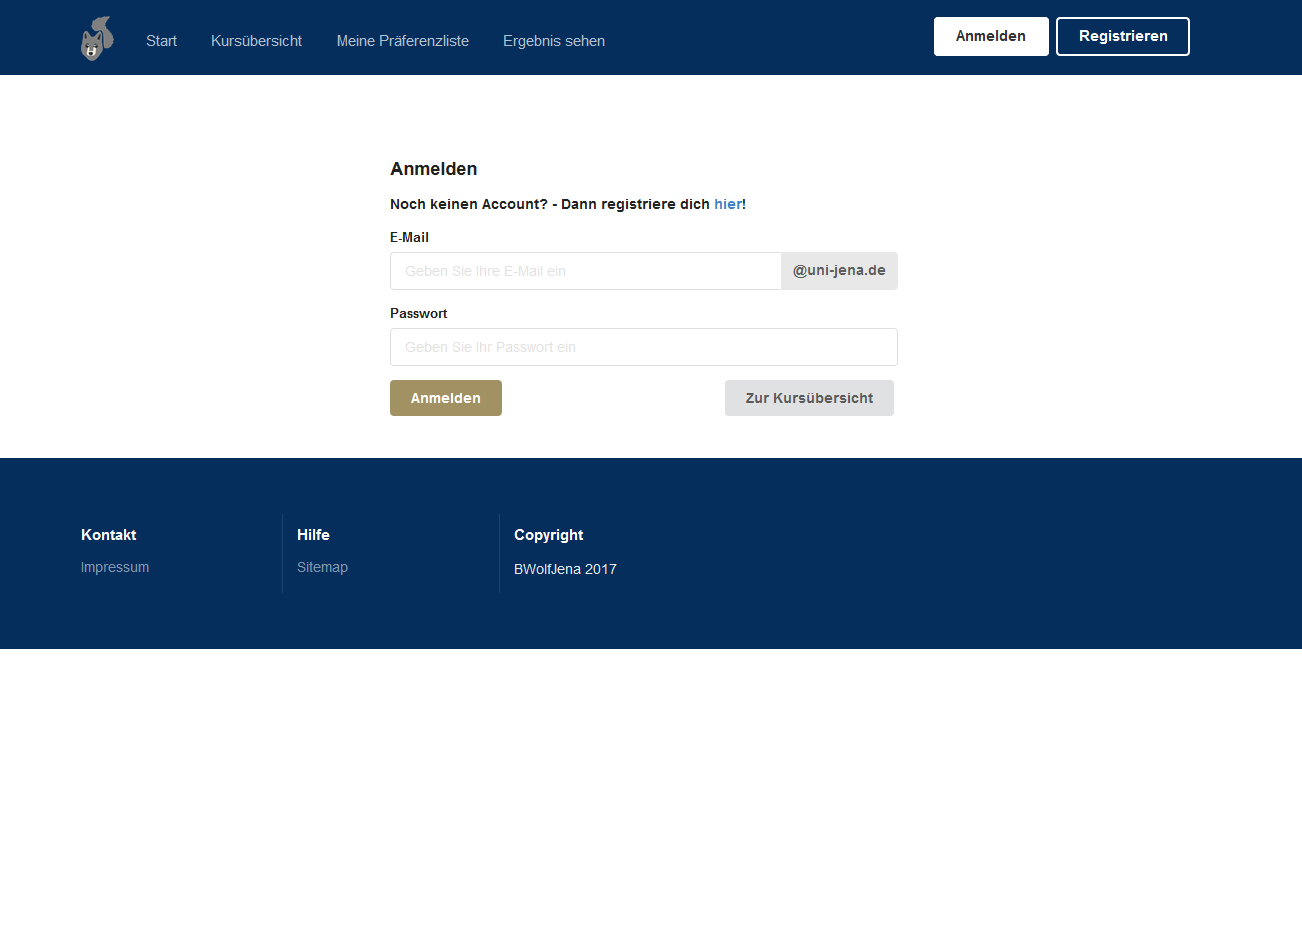
\includegraphics[width=1.0\textwidth]{./implementation/images/login.png}
            \end{subfigure}
            \caption{Gegenüberstellung von Entwurf der Login-Oberfläche (links) und Umsetzung (rechts)}
            \label{fig:comparisonLogin}
        \end{figure}
    
        In Abbildung \ref{fig:comparisonLogin} sind der Entwurf für die Login-Oberfläche und die Umsetzung selbiger gegenüber gestellt.
        Es fällt auf, dass die grobe Struktur der Seite bis auf kleine Änderungen mit dem Entwurf übereinstimmt.
        Unterschiede lassen sich vor allem in der Kopfzeile erkennen.
        So wurde der Reiter \textit{Start} hinzugefügt.
        Anders als zuvor angedacht, fiel die Entscheidung für eine Startseite, in der das Empiriepraktikum kurz vorgestellt wird.
        Des Weiteren wurde der Reiter \textit{Einschreiben} aus Gründen der Verständlichkeit in \textit{Meine Präferenzliste} umbenannt.
        Die Seite erfüllt jedoch die selbe Funktion.
    
        \begin{figure}
            \centering
            \begin{subfigure}{0.4\textwidth}
                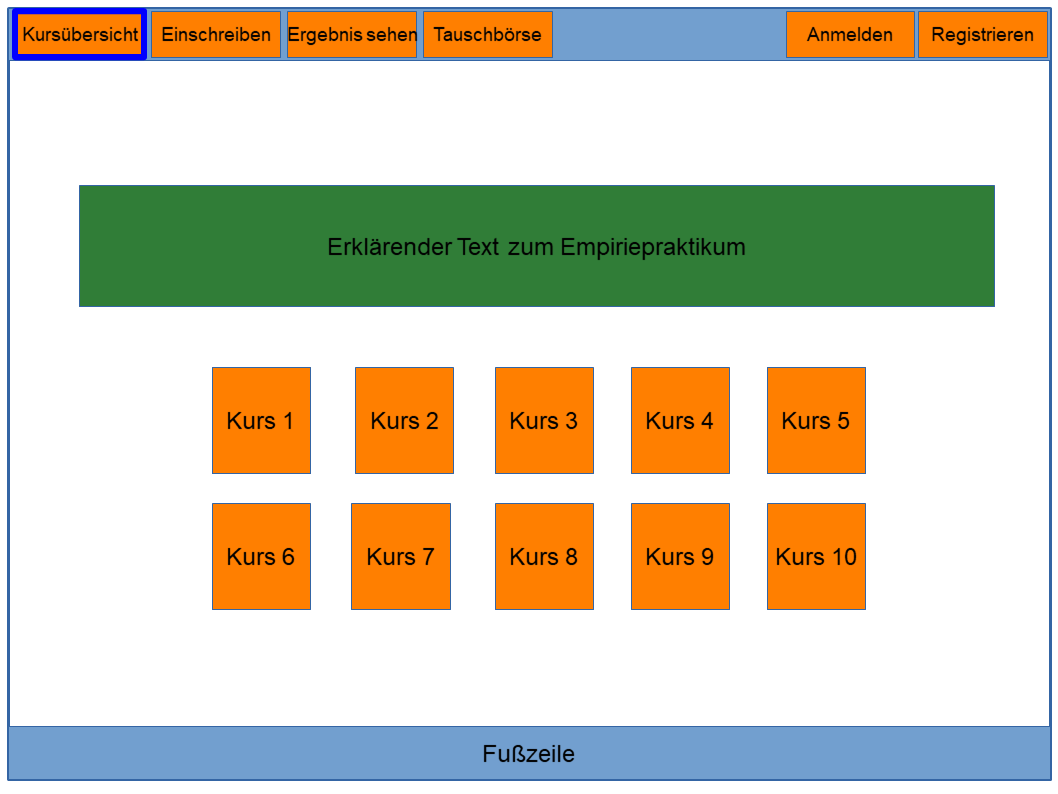
\includegraphics[width=1.0\textwidth]{./implementation/images/MockUpsFrontend/frontendCourses.png}
            \end{subfigure}
            \begin{subfigure}{0.59\textwidth}
                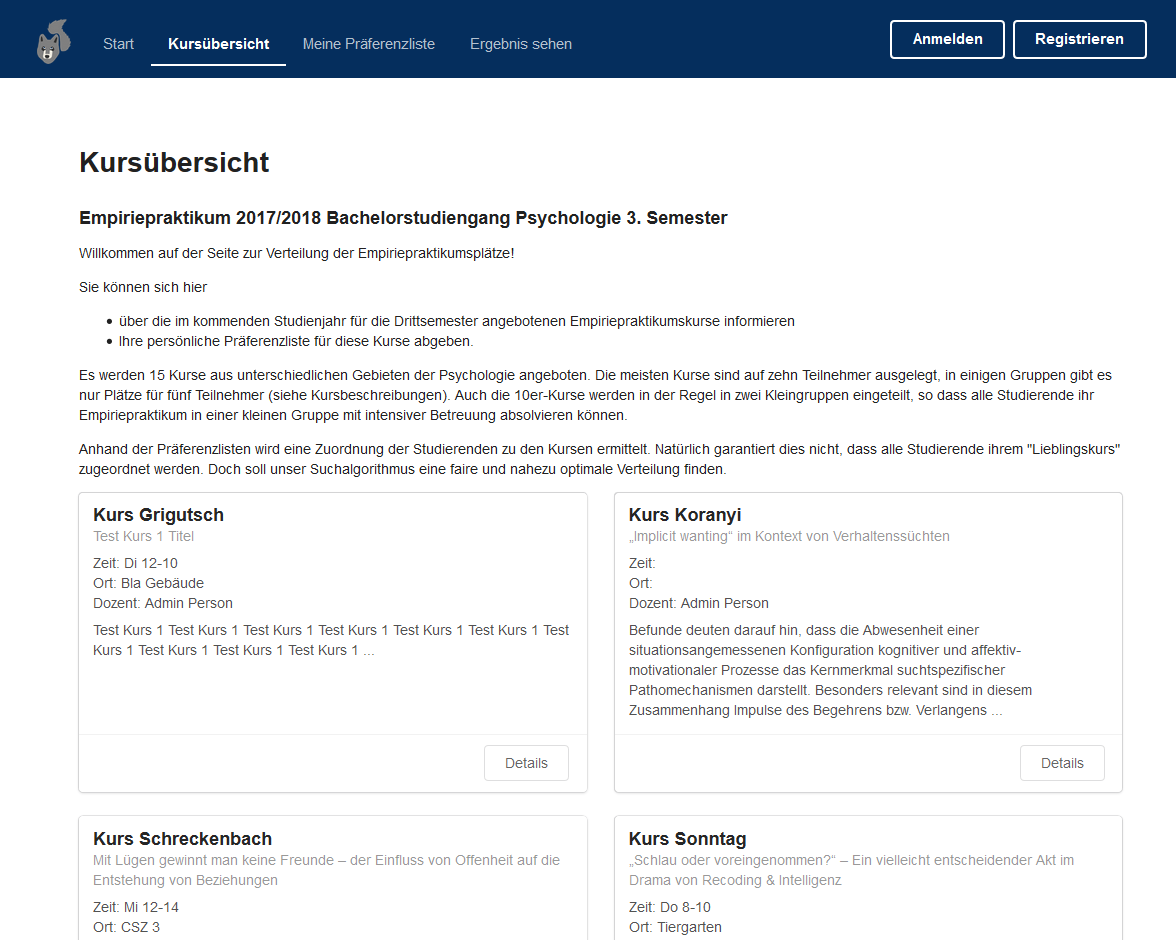
\includegraphics[width=1.0\textwidth]{./implementation/images/courses.png}
            \end{subfigure}
            \caption{Gegenüberstellung von Entwurf der Kursübersicht (links) und Umsetzung (rechts)}
            \label{fig:comparisonCourses}
        \end{figure}
    
        Abbildung \ref{fig:comparisonCourses} zeigt Entwurf und Umsetzung der Kursübersicht.
        Die Struktur des Entwurfs wurde direkt umgesetzt.
        Wie in Kapitel \ref{chapter:requirements} beschrieben, ist es, wie in Abbildung \ref{fig:comparisonCourses} zu sehen ist, möglich auch ohne eine Anmeldung auf die Kursübersicht zuzugreifen.
        Es ist anzumerken, dass die Fußleiste auch in der Kursübersicht \ref{fig:comparisonCourses} den Abschluss der Seite bildet und lediglich durch die Menge an Kursen nicht zu sehen ist.
        
        \begin{figure}
            \centering
            \begin{subfigure}{0.4\textwidth}
                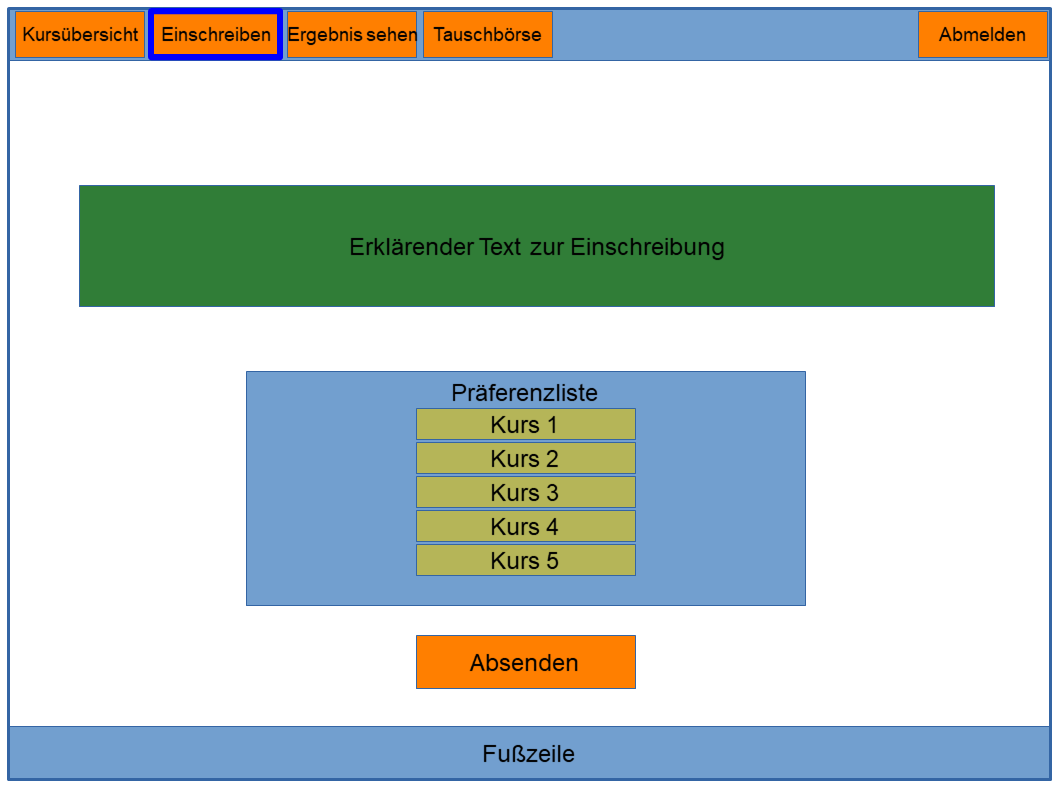
\includegraphics[width=1.0\textwidth]{./implementation/images/MockUpsFrontend/frontendPreferences.png}
            \end{subfigure}
            \begin{subfigure}{0.59\textwidth}
                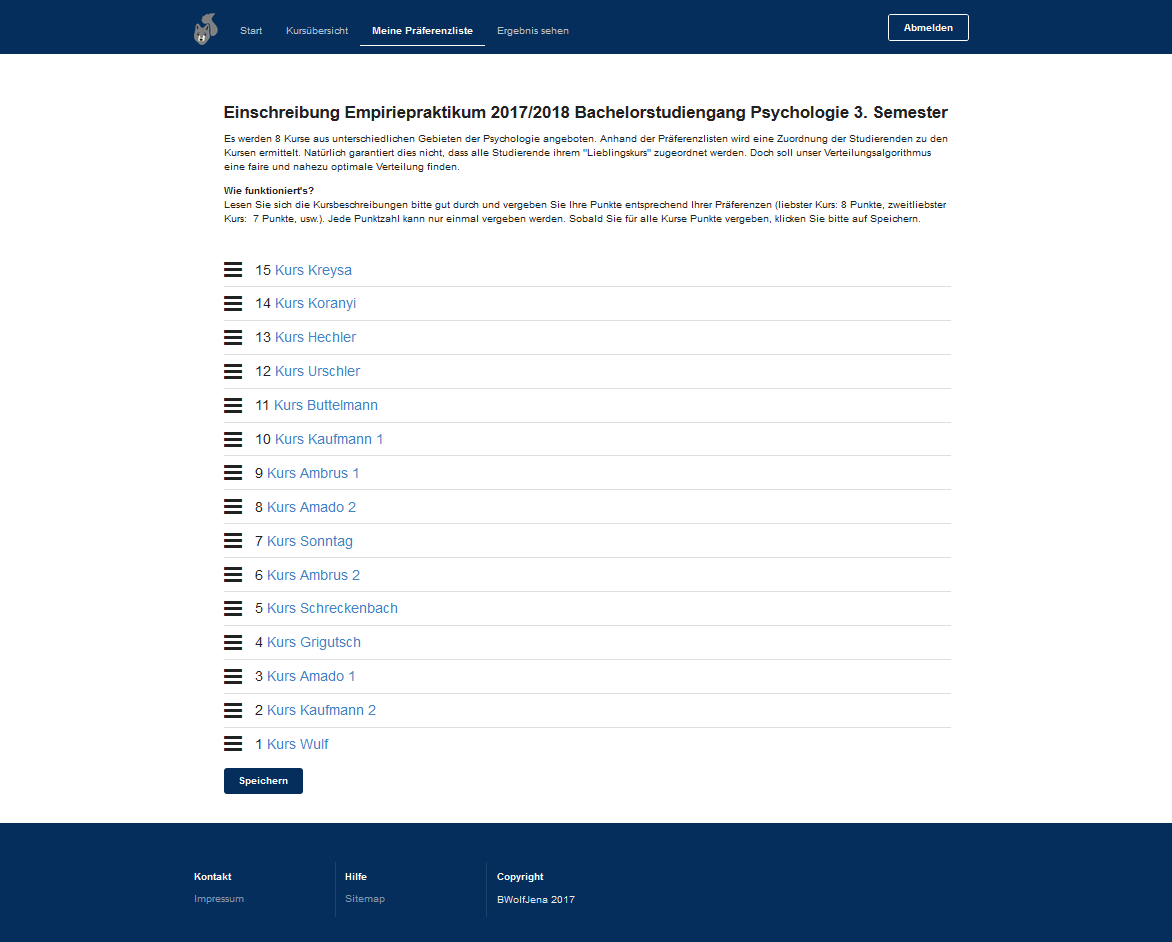
\includegraphics[width=1.0\textwidth]{./implementation/images/preferences.png}
            \end{subfigure}
            \caption{Gegenüberstellung von Entwurf der Einschreibungs-Oberfläche (links) und Umsetzung (rechts)}
            \label{fig:comparisonPrefenrences}
        \end{figure}
    
        Die Oberfläche zum Erstellen der Präferenzliste wurde ebenfalls wie angedacht umgesetzt.
        Mithilfe von Drag\&Drop könne die verschiedenen Kurse in die gewünschte Reihenfolge gebracht werden.
        Der Knopf \textit{Absenden} wurde in \textit{Speichern} umbenannt.
        Dadurch soll mehr Klarheit darüber geschaffen werden, dass die Präferenzliste bis zum Ablauf der Frist jederzeit verändert werden kann.\\
        
        Es ist zu erwähnen, dass das gesamte Frontend auch auf mobilen Geräten unterstützt wird.
        Die Ansichten für Kursübersicht und auch die Wahl der Präferenzliste werden entsprechend der Größe des Bildschirms angepasst, sodass die Benutzerfreundlichkeit erhalten bleibt.\\
        
        Die Tauschbörse wurde nicht implementiert.
        Grund hierfür ist zum einen die zeitliche Beschränkung des Projekts, wodurch einige optionale Funktionalitäten nicht umgesetzt werden konnten.
        Zum anderen sind bei einem weiteren Gespräch nach dem Erstellen der Anforderungen Zweifel an der Notwendigkeit solch einer Tauschbörse aufgetreten.
        Eine weitere Funktion, die nicht im Frontend umgesetzt werden konnte, war die in Kapitel \ref{chapter:design} geplante Erweiterbarkeit auf andere Module.
        So kann ein Benutzer im Frontend nicht mehrere Präferenzlisten parallel verwalten.\\
        
        Im Frontend wurde jedoch auch eine zusätzliche Funktionalität implementiert.
        So wurde ein Archiv umgesetzt, in dem die Kurse vergangener Empiriepraktika einsehbar sind.
    
    \section{Backend}
        Auch im Backend ist die Struktur der Entwürfe weitestgehend übernommen worden.
        
        \begin{figure}
            \centering
            \begin{subfigure}{0.4\textwidth}
                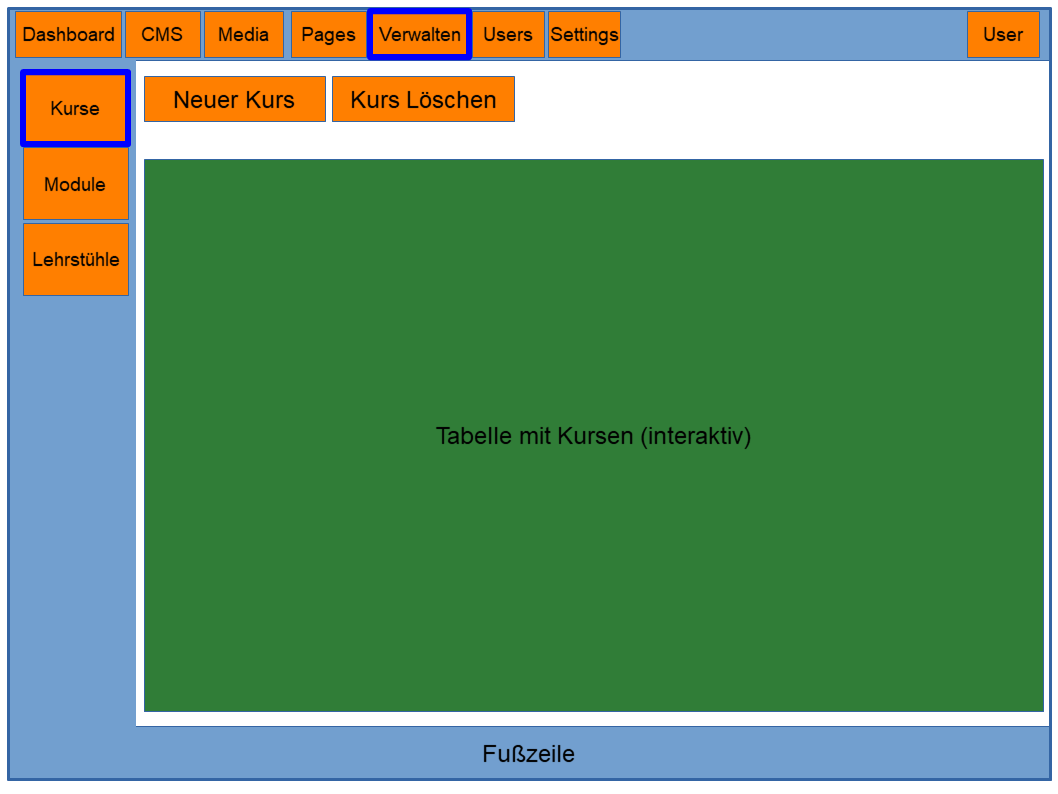
\includegraphics[width=1.0\textwidth]{./implementation/images/MockUpsBackend/backendManageCourses.png}
            \end{subfigure}
            \begin{subfigure}{0.59\textwidth}
                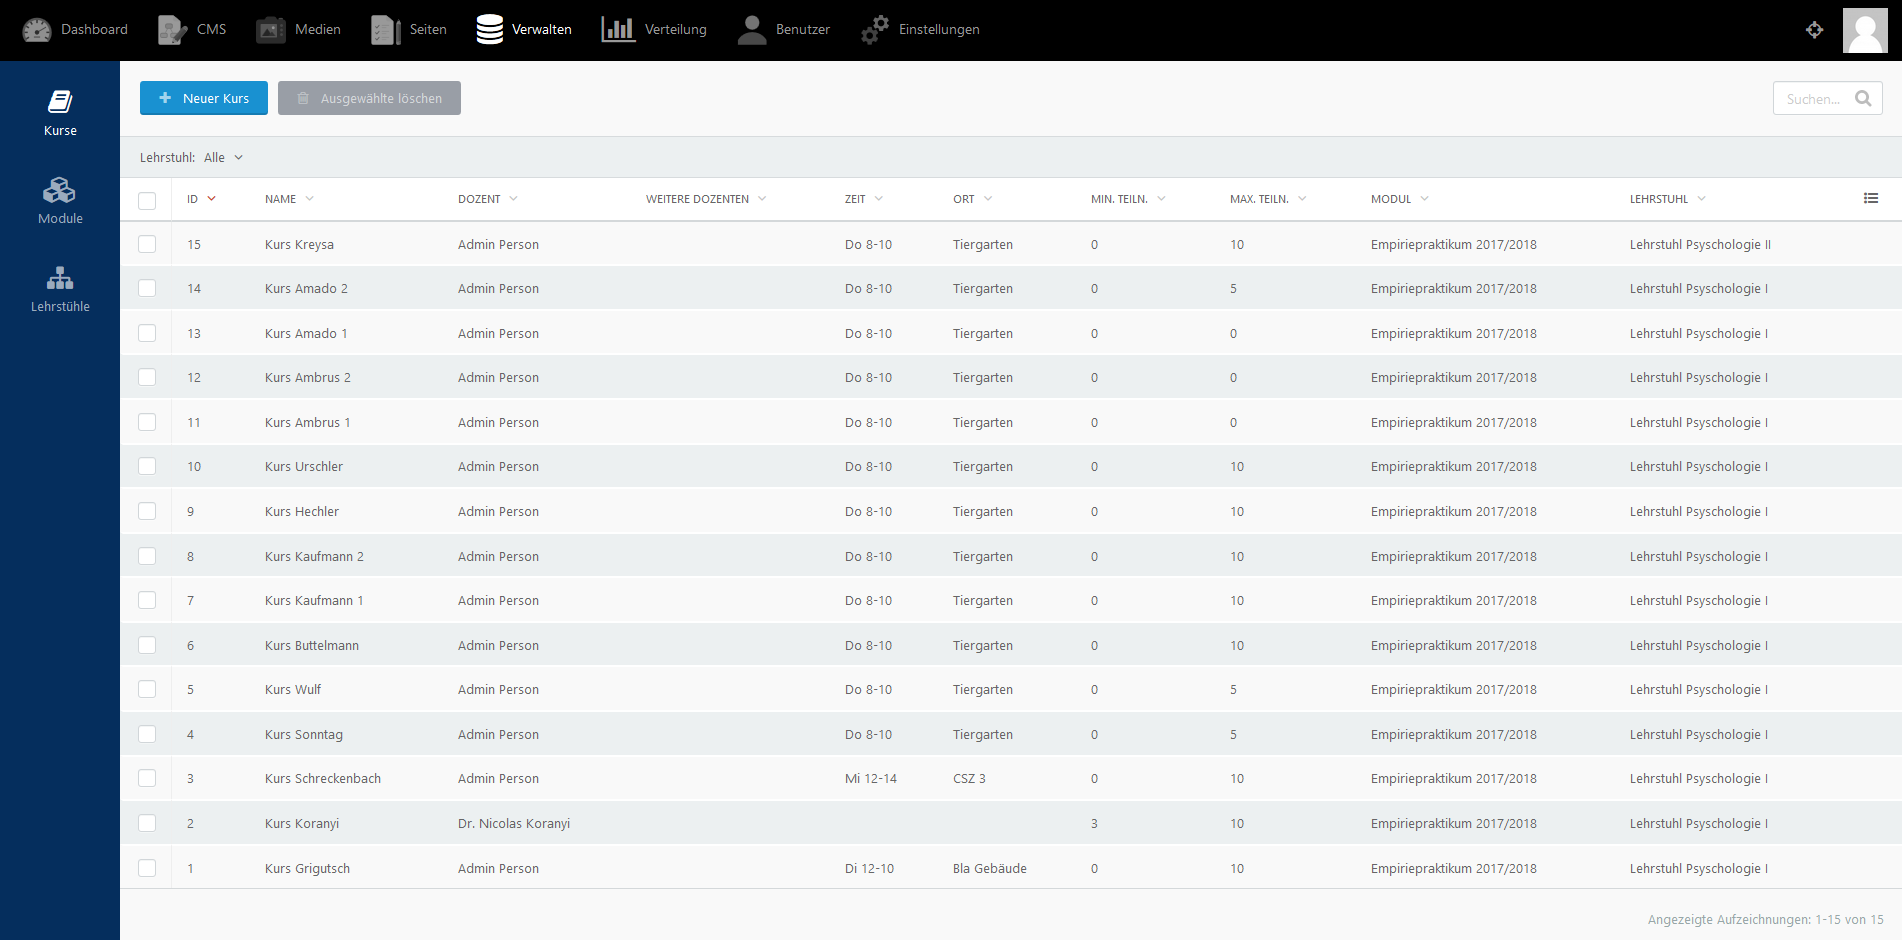
\includegraphics[width=1.0\textwidth]{./implementation/images/manageCourses.png}
            \end{subfigure}
            \caption{Gegenüberstellung von Entwurf der Kursverwaltung (links) und Umsetzung (rechts)}
            \label{fig:comparisonManageCourses}
        \end{figure}
        
        Abbildung \ref{fig:comparisonManageCourses} zeigt Entwurf und Umsetzung der Kursverwaltung.
        Die Struktur aus Kopf- und Seitenleiste wurde übernommen.
        Die Fußzeile wurde jedoch entfernt.
        Es fällt außerdem auf, dass die Kopfzeile mehr Reiter umfasst, als zunächst geplant.
        Das zum Erstellen des Backend verwendete Framework \textit{October CMS} stellt einige vordefinierte Seiten zur Verfügung.
        Darunter fällt das \textit{Dashboard}, in dem zum Start des Backends einige wichtige Informationen angezeigt werden.
        Unter dem Reiter \textit{Seiten} können weiter Seiten für das Frontend erstellt und die vorhanden Seiten bearbeitet werden.
        Im Entwurf wurde an diese wichtige Funktion des Backends nicht gedacht und so wurde dieser von \textit{October CMS} bereitgestellte \todo{Dienst} übernommen.
        Der Reiter \textit{Einstellungen} ist ebenfalls von \textit{October CMS} bereitgestellt und erlaubt das Andern und Verwalten verschiedenste Optionen.
        Für dieses Projekt relevant sind vor allem die Einstellungen bezüglich der automatisch versendeten E-Mails, sowie das Verwalten der Backendbenutzer.
        Anders als im Entwurf vorgesehen, werden nicht alle Benutzer über den Reiter \textit{Benutzer} verwaltet, sondern nur die Frontendnutzer.
        Diese Änderung ist durch \textit{October CMS} bedingt.
        
        \begin{figure}
            \centering
            \begin{subfigure}{0.4\textwidth}
                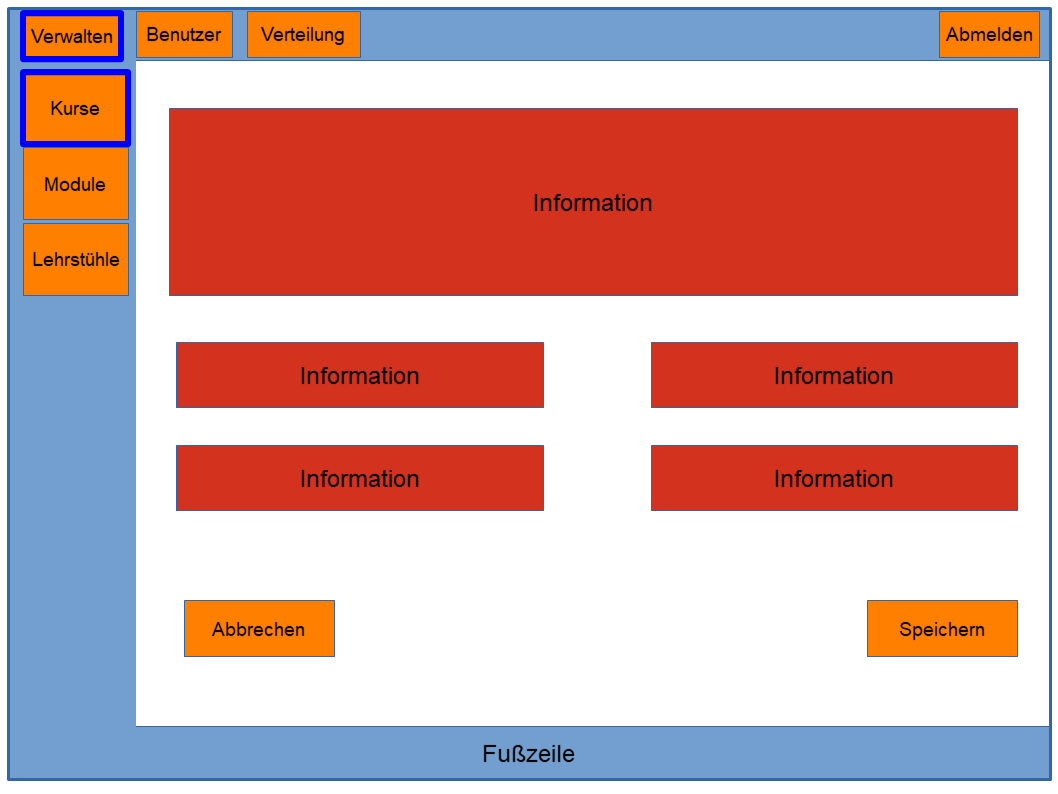
\includegraphics[width=1.0\textwidth]{./implementation/images/MockUpsBackend/backendEdit.png}
            \end{subfigure}
            \begin{subfigure}{0.59\textwidth}
                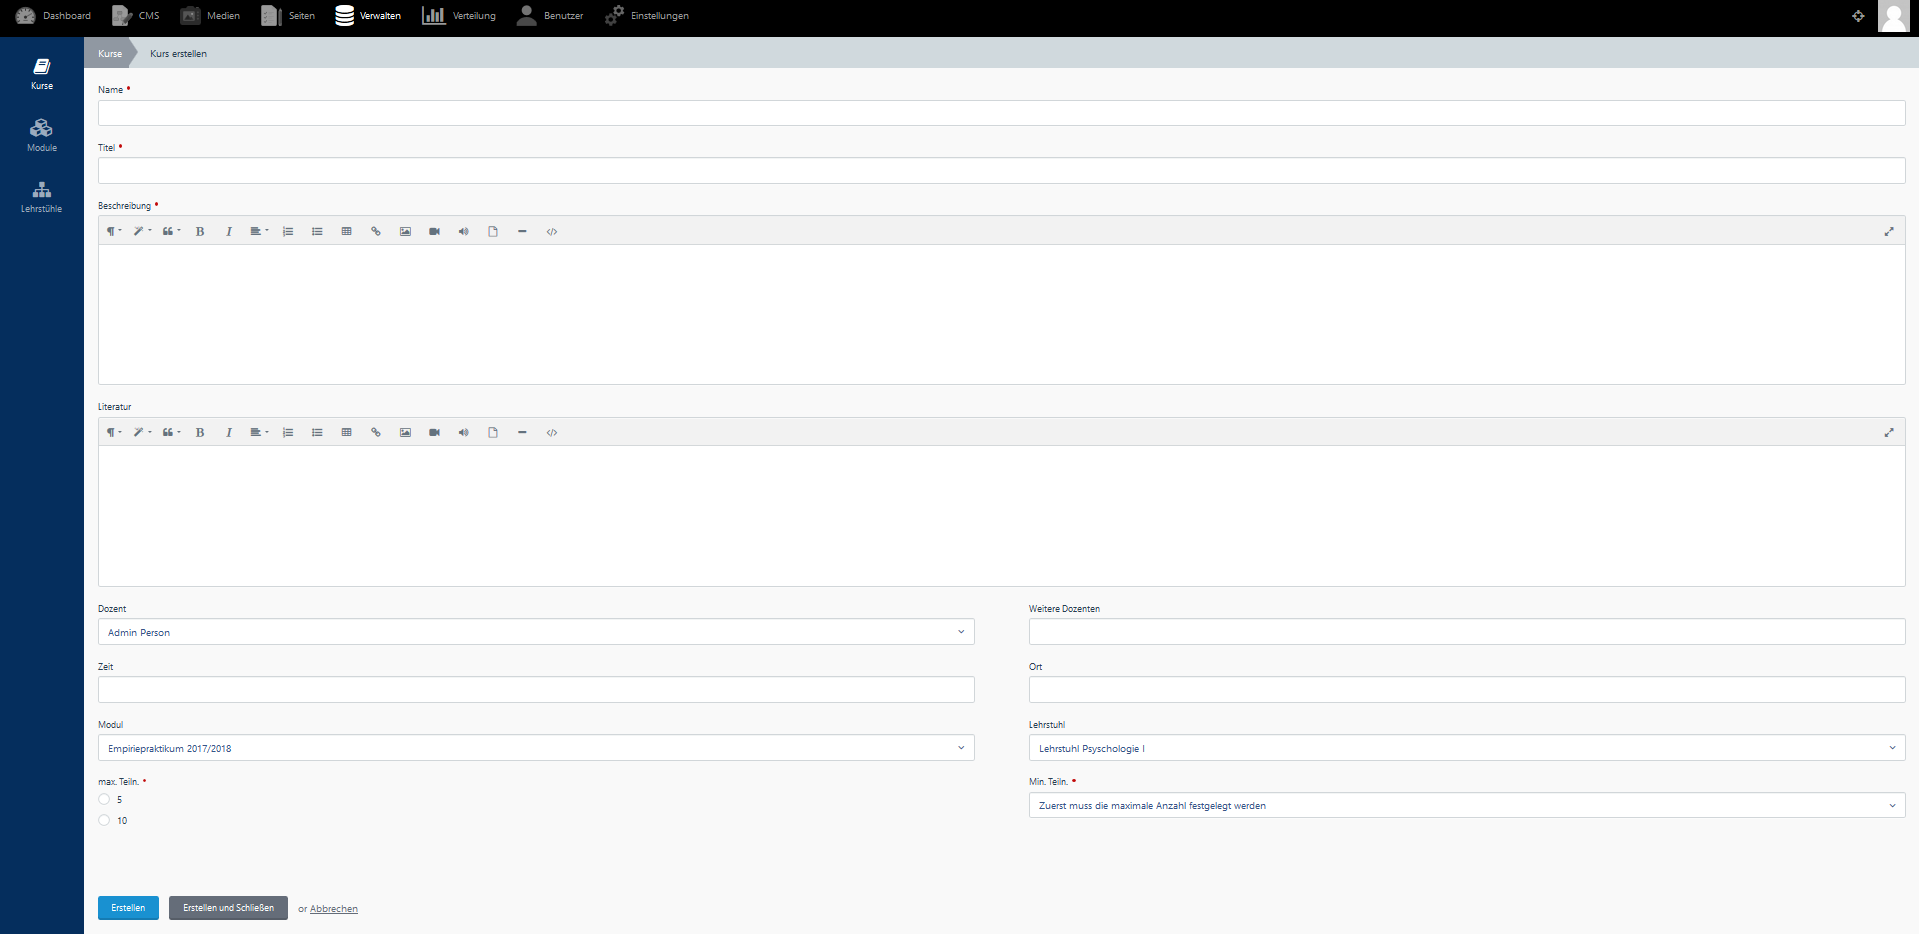
\includegraphics[width=1.0\textwidth]{./implementation/images/edit.png}
            \end{subfigure}
            \caption{Gegenüberstellung von Entwurf der Kurserstellung (links) und Umsetzung (rechts)}
            \label{fig:comparisonEdit}
        \end{figure}
    
        Das Erstellen und bearbeiten von Kursen, Lehrstühlen, Benutzern, usw. ist, wie in Abbildung \ref{fig:comparisonEdit} zu sehen, wie im Entwurf umgesetzt.
        Verschiedene Eingabefelder mit \textit{Richtext}-Bearbeitung und Auswahlfelder werden wie vorgesehen zur Verfügung gestellt.
    
        \begin{figure}
            \centering
            \begin{subfigure}{0.4\textwidth}
                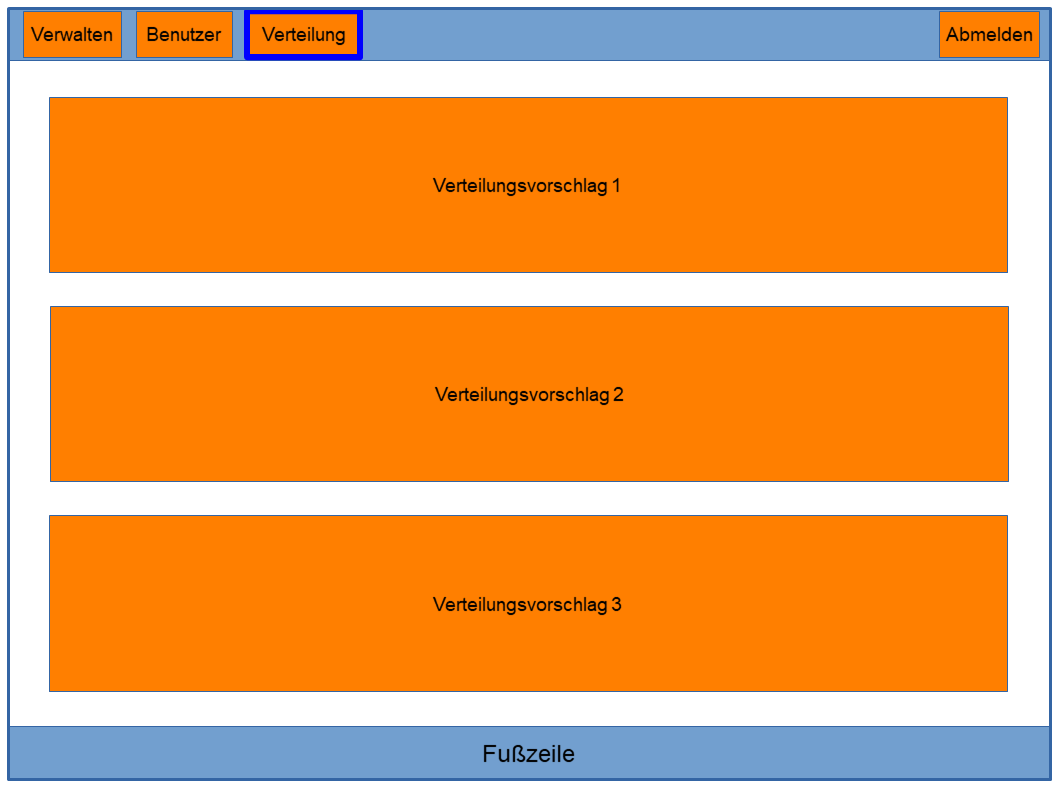
\includegraphics[width=1.0\textwidth]{./implementation/images/MockUpsBackend/backendDistribution.png}
            \end{subfigure}
            \begin{subfigure}{0.59\textwidth}
                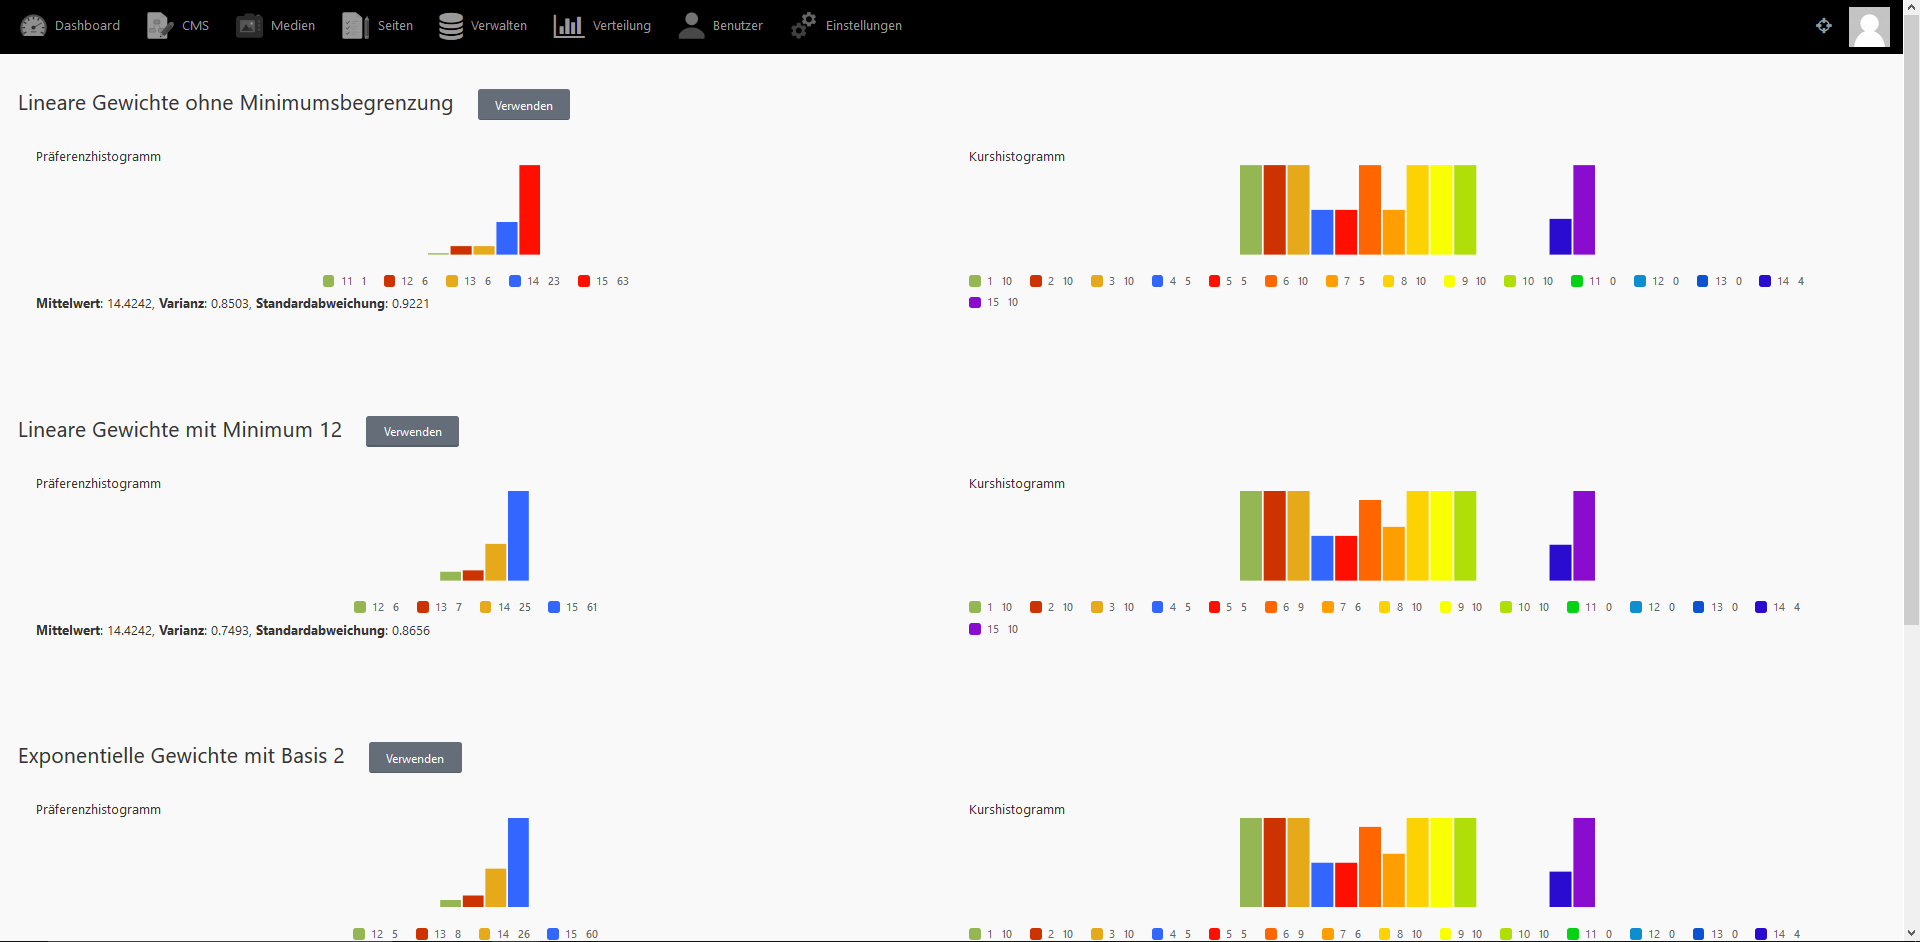
\includegraphics[width=1.0\textwidth]{./implementation/images/distribution.png}
            \end{subfigure}
            \caption{Gegenüberstellung von Entwurf der Anzeige der Verteilungsvorschläge (links) und Umsetzung (rechts)}
            \label{fig:comparisonDistribution}
        \end{figure}
    
        Auch der Entwurf der Verteilungsansicht wurde umgesetzt.
        In Abbildung \ref{fig:comparisonDistribution} sind wieder Mockup und Resultat gegenübergestellt.
        Die genaue Umsetzung des Verteilungsalgorithmus wird im nächsten Kapitel näher erläutert.
        